% =====================================================================
%  IN6049 --- Forecasting and Regression Analysis
%  Week 8: Logistic Regression, Poisson Regression and GLMs --- Tips dataset
%
%  Built from template/slides-template.tex (Boadilla + seahorse, 16:9).
%  Title slide + 2 recap slides + 7 week-8 slides.  Numbers come from
%  Assigment_8.ipynb; figures are its exported PNGs (images/ -> fig_*.png here).
%
%  Compiles on Overleaf with the default pdfLaTeX engine.
%  Upload alongside: fig_bands.png , fig_smoker.png , fig_by_day.png ,
%  fig_diag.png , fig_roc.png , fig_poisson.png
% =====================================================================
\documentclass[aspectratio=169,11pt]{beamer}

\usetheme{Boadilla}
\usecolortheme{seahorse}
\setbeamertemplate{navigation symbols}{}

\usepackage[utf8]{inputenc}
\usepackage[T1]{fontenc}
\usepackage{booktabs}
\usepackage{amsmath}
\usepackage{graphicx}
\usepackage{url}

% Emphasis lead-in: bold + structure colour.  Use as \key{Finding.} text...
\newcommand{\key}[1]{\textbf{\structure{#1}}}

% Figure placeholder, so the template compiles with no image files.
% Replace each use by  \includegraphics[width=0.9\linewidth]{@@ file @@}
% (vector PDF preferred; PNG is fine).
\newcommand{\figbox}[2]{%
  \fbox{\parbox[c][#2][c]{#1}{\centering\scriptsize\color{gray}@@ figure @@}}}

% ---------------------------------------------------------------------
\title[Logistic and Poisson regression]{Logistic Regression, Poisson Regression and GLMs --- Tips}
\subtitle{Modelling a yes/no response: does the party smoke?}
\author[Jie Dong, Elivier Reyes]{Jie Dong, Elivier Reyes}
\date[IN6049]{}

\begin{document}

% ===================== TITLE ========================================
\begin{frame}
  \titlepage
  \vspace{-1.2em}
  \begin{center}
    \small\urlstyle{same}\url{https://github.com/HelloJJJie/Assignment-Forecast-and-Analysis-of-Regression.git}

    \vspace{1.2em}
    $n=244$ parties, $93$ of them smokers ($38\%$): what do the bill, the
    party size and the day say about smoking status?
  \end{center}
\end{frame}

% ===================== RECAP 1 ======================================
\begin{frame}{Recap 1. Linear regression for a continuous response (weeks 1--5)}
  \begin{columns}[T]
  \begin{column}{0.54\textwidth}
    \small
    \begin{itemize}
      \item \key{Simple regression:} tip $=0.920+0.105\,$bill, $R^2=0.457$,
            $F^{*}=203.4$; a family $95\%$ interval for $\beta_0,\beta_1$ needs
            multiplier $2.255$ (Bonferroni), not $1.970$.
      \item \key{Diagnostics:} constant variance and normality are rejected
            (Breusch--Pagan $P=4\times10^{-21}$).
      \item \key{Multiple regression, hat matrix:} bill and size give
            $R^2=0.468$; leverage $h_{ii}>2p/n$ for $22$ of $244$ cases.
      \item \key{Partial tests, multicollinearity:} $SSR(X_2\mid X_1)=5.2$
            but $SSR(X_2\mid X_3)=145.3$; with bill per person
            $VIF=17.3,\,10.4,\,11.4$.
      \item \key{Indicators:} only \emph{smoker} changes the line
            (slopes $0.137$ vs.\ $0.070$).
    \end{itemize}
  \end{column}
  \begin{column}{0.46\textwidth}
    \centering
    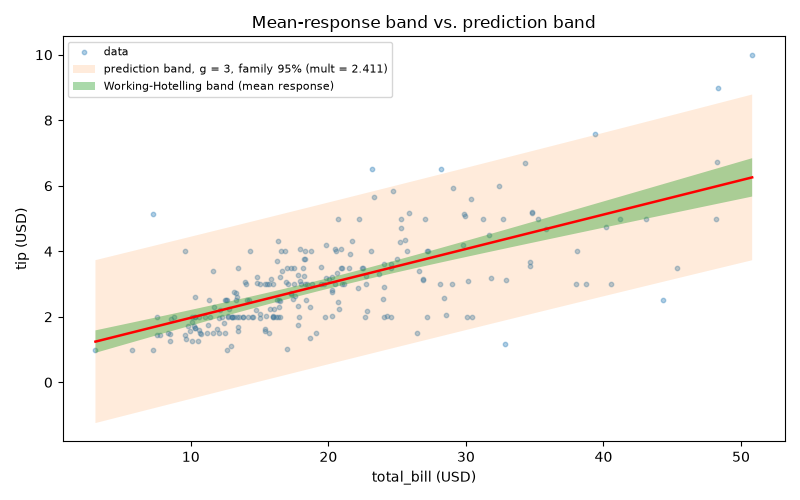
\includegraphics[width=0.88\linewidth]{fig_bands.png}

    \vspace{-0.1em}
    {\scriptsize Fit with confidence and prediction bands: a continuous response.}
  \end{column}
  \end{columns}
\end{frame}

% ===================== RECAP 2 ======================================
\begin{frame}{Recap 2. Selecting and checking the model (weeks 6--7)}
  \begin{columns}[T]
  \begin{column}{0.54\textwidth}
    \small
    \begin{itemize}
      \item \key{Selection:} of $128$ subsets, $R^2_a$, $C_p$, $AIC$, $SBC$ and
            $PRESS$ all pick \{bill, smoker, bill$\times$smoker\}; three stepwise
            paths agree; mean MSPR $1.034$ vs.\ $1.084$ (bill only).
      \item \key{Diagnostics:} one influential case, row $170$
            ($t=5.65$, Cook's $D=0.893$); without it the smokers' slope
            falls from $0.070$ to $0.051$.
      \item \key{Remedies:} weighted least squares flattens the funnel (not
            fully); bootstrap and HC3 standard errors ($0.0232$, $0.0255$) exceed
            the ordinary $0.0142$ for the interaction.
    \end{itemize}

    \vspace{0.2em}
    \key{This week:} the response is a \emph{yes/no}.
  \end{column}
  \begin{column}{0.46\textwidth}
    \centering
    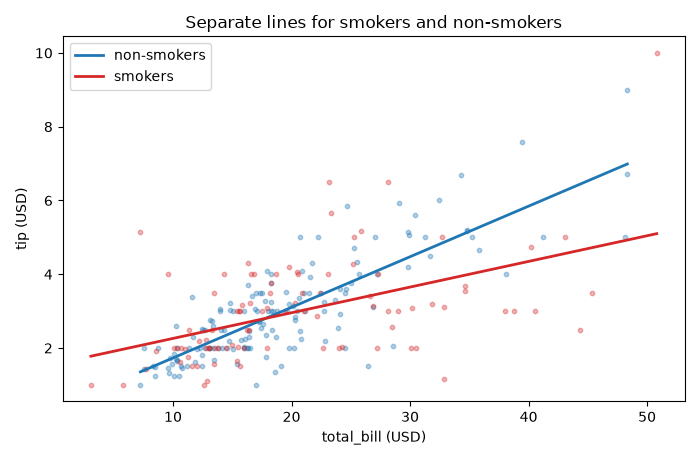
\includegraphics[width=0.90\linewidth]{fig_smoker.png}

    \vspace{-0.1em}
    {\scriptsize One line per smoking status: smoking was a \emph{predictor} so far;
     now it becomes the response.}
  \end{column}
  \end{columns}
\end{frame}

% ===================== 1. WHY NOT OLS ===============================
\begin{frame}{1. Why not ordinary regression? Odds and the logit}
  \begin{columns}[T]
  \begin{column}{0.54\textwidth}
    \small
    $Y=1$ if smoker; $E\{Y\mid X\}=\pi(X)$, $Var\{Y\}=\pi(1-\pi)$, two-valued error.
    Linear probability fit (bill, size, day):

    \vspace{0.2em}
    \begin{itemize}
      \item fitted values $-0.012$ to $0.954$: $2$ cases outside $[0,1]$;
      \item $Var\{Y\}$ depends on $X$ in theory; Breusch--Pagan detects nothing in these residuals ($P=0.55$).
    \end{itemize}

    \vspace{0.2em}
    \key{Logistic model:}
    $\pi=\dfrac{1}{1+e^{-\eta}}$, $\ \mathrm{logit}(\pi)=\ln\dfrac{\pi}{1-\pi}=\eta$, $\ OR_k=e^{\beta_k}$.

    \vspace{0.1em}
    {\scriptsize
    \begin{tabular}{@{}rrr@{\hskip 2em}rrr@{}}
      \toprule
      $\pi$ & odds & logit & $\pi$ & odds & logit \\
      \midrule
      $0.10$ & $0.11$ & $-2.20$ & $0.75$ & $3.00$ & $+1.10$ \\
      $0.25$ & $0.33$ & $-1.10$ & $0.90$ & $9.00$ & $+2.20$ \\
      $0.50$ & $1.00$ & $0.00$  &        &        &        \\
      \bottomrule
    \end{tabular}}
  \end{column}
  \begin{column}{0.46\textwidth}
    \centering
    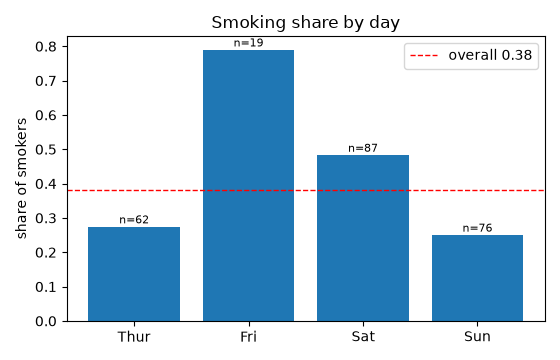
\includegraphics[width=0.88\linewidth]{fig_by_day.png}

    \vspace{-0.1em}
    {\scriptsize Share of smokers: Friday $0.79$ (only $19$ parties), Saturday
     $0.48$, Sunday $0.25$, Thursday $0.27$. Larger parties smoke less:
     $0.42$ (size 2), $0.30$ (size 4), $0/4$ (size 6).}
  \end{column}
  \end{columns}
\end{frame}

% ===================== 2. MAXIMUM LIKELIHOOD ========================
\begin{frame}{2. Maximum likelihood and the odds ratio}
  \begin{columns}[T]
  \begin{column}{0.52\textwidth}
    \small
    No least-squares formula: Newton--Raphson (IRLS),
    $\mathbf b\leftarrow\mathbf b+(\mathbf X'\mathbf W\mathbf X)^{-1}\mathbf X'(\mathbf y-\boldsymbol\mu)$,
    $\widehat{Var}\{\mathbf b\}=(\mathbf X'\mathbf W\mathbf X)^{-1}$. Written by hand,
    equal to \texttt{statsmodels}. Smoker on party size:

    \vspace{0.3em}
    {\scriptsize
    \begin{tabular}{@{}rrr@{}}
      \toprule
      iteration & $\ln L$ & max $|$step$|$ \\
      \midrule
      $1$ & $-159.9445$ & $2.7\times10^{-1}$ \\
      $2$ & $-159.8998$ & $7.9\times10^{-2}$ \\
      $3$ & $-159.8998$ & $1.9\times10^{-3}$ \\
      $5$ & $-159.8998$ & $2.7\times10^{-13}$ \\
      \bottomrule
    \end{tabular}}

    \vspace{0.3em}
    $\mathrm{logit}(\hat\pi)=0.306-0.3126\,\mathrm{size}$;
    $\ln L_{null}=-162.168$.
  \end{column}
  \begin{column}{0.48\textwidth}
    \small
    \begin{itemize}
      \item \key{Odds ratio:} $e^{b_1}=0.732$ per extra person, $95\%$ CI
            $(0.543,\,0.986)$: each person lowers the odds of a smoking party by $27\%$.
      \item \key{Wald:} $z^{*}=-2.05$, $P=0.040$.
      \item \key{Likelihood ratio:} $G^2=4.54$, df $1$, $P=0.033$ (agrees).
      \item McFadden $R^2=0.014$: size alone explains almost nothing.
    \end{itemize}

    \vspace{0.3em}
    {\scriptsize
    \begin{tabular}{@{}lrrrrrr@{}}
      \toprule
      size & 1 & 2 & 3 & 4 & 5 & 6 \\
      \midrule
      fitted $\hat\pi$ & $.50$ & $.42$ & $.35$ & $.28$ & $.22$ & $.17$ \\
      observed         & $.50$ & $.42$ & $.32$ & $.30$ & $.40$ & $0$ \\
      $n$              & 4 & 156 & 38 & 37 & 5 & 4 \\
      \bottomrule
    \end{tabular}}
  \end{column}
  \end{columns}
\end{frame}

% ===================== 3. MULTIPLE LOGISTIC =========================
\begin{frame}{3. Multiple logistic regression and likelihood-ratio tests}
  \begin{columns}[T]
  \begin{column}{0.58\textwidth}
    \small
    $\mathrm{logit}(\pi)=\beta_0+\beta_1\mathrm{bill}+\beta_2\mathrm{size}+\beta_3\mathrm{Sat}+\beta_4\mathrm{Sun}+\beta_5\mathrm{Thur}$
    (Friday = baseline). Adjusted odds ratios:

    \vspace{0.3em}
    {\scriptsize\setlength{\tabcolsep}{3pt}
    \begin{tabular}{@{}lrrrrrl@{}}
      \toprule
       & $b$ & $s\{b\}$ & $z^{*}$ & $P$ & $OR$ & $95\%$ CI \\
      \midrule
      bill   & $0.0621$  & $0.0205$ & $3.03$  & $0.0024$ & $1.064$ & $(1.022,\,1.108)$ \\
      size   & $-0.590$  & $0.211$  & $-2.79$ & $0.0052$ & $0.554$ & $(0.366,\,0.839)$ \\
      Sat    & $-1.396$  & $0.615$  & $-2.27$ & $0.023$  & $0.248$ & $(0.074,\,0.827)$ \\
      Sun    & $-2.360$  & $0.642$  & $-3.68$ & $0.0002$ & $0.094$ & $(0.027,\,0.332)$ \\
      Thur   & $-2.210$  & $0.640$  & $-3.46$ & $0.0005$ & $0.110$ & $(0.031,\,0.384)$ \\
      \bottomrule
    \end{tabular}}
  \end{column}
  \begin{column}{0.42\textwidth}
    \small
    \key{Likelihood-ratio tests} (drop a term):

    \vspace{0.2em}
    {\scriptsize
    \begin{tabular}{@{}lrrr@{}}
      \toprule
       & $G^2$ & df & $P$ \\
      \midrule
      bill & $9.70$  & $1$ & $0.0018$ \\
      size & $8.78$  & $1$ & $0.0031$ \\
      day  & $22.16$ & $3$ & $6\times10^{-5}$ \\
      whole model & $37.60$ & $5$ & $4.6\times10^{-7}$ \\
      \bottomrule
    \end{tabular}}

    \vspace{0.4em}
    \small
    Holding size and day fixed, each extra dollar raises the odds by $6\%$;
    every Sunday party has $9\%$ of a Friday party's odds. Friday is
    $19$ parties, so its baseline is imprecise (wide intervals).
  \end{column}
  \end{columns}
\end{frame}

% ===================== 4. SELECTION AND FIT =========================
\begin{frame}{4. Model selection and goodness of fit}
  \begin{columns}[T]
  \begin{column}{0.54\textwidth}
    \small
    $AIC=-2\ln L+2p$, $SBC=-2\ln L+p\ln n$; $32$ subsets of five terms
    (\texttt{day} as one group):

    \vspace{0.2em}
    {\scriptsize\setlength{\tabcolsep}{3pt}
    \begin{tabular}{@{}lrrrrr@{}}
      \toprule
      model & $p$ & $AIC$ & $\Delta AIC$ & $SBC$ & $\Delta SBC$ \\
      \midrule
      bill, size, day          & $6$ & $298.74$ & $0.00$ & $319.72$ & $0.00$ \\
      + dinner                 & $7$ & $299.56$ & $0.82$ & $324.04$ & $4.32$ \\
      + male                   & $7$ & $300.73$ & $1.99$ & $325.21$ & $5.49$ \\
      bill, day                & $5$ & $305.51$ & $6.78$ & $323.00$ & $3.28$ \\
      day                      & $4$ & $306.37$ & $7.63$ & $320.36$ & $0.64$ \\
      \bottomrule
    \end{tabular}}

    \vspace{0.3em}
    AIC and SBC both choose \{bill, size, day\}.
  \end{column}
  \begin{column}{0.46\textwidth}
    \small
    \begin{itemize}
      \item \key{Hosmer--Lemeshow} ($10$ groups of $\hat\pi$): $\chi^2=5.34$,
            $8$ df ($g-2$, the standard choice; the slide gives no df),
            $P=0.72$: no evidence of lack of fit.
      \item \key{Deviance} $D=-2\ln L=286.7$ on $238$ df is \emph{not} read as a
            $\chi^2$ test: ungrouped $0/1$ data.
      \item \key{McFadden} $R^2=0.116$: below the $0.2$--$0.4$ range of a good fit.
            The model fits but does not predict smoking well.
    \end{itemize}
  \end{column}
  \end{columns}
\end{frame}

% ===================== 5. DIAGNOSTICS ===============================
\begin{frame}{5. Residuals, leverage and influence}
  \begin{columns}[T]
  \begin{column}{0.56\textwidth}
    \centering
    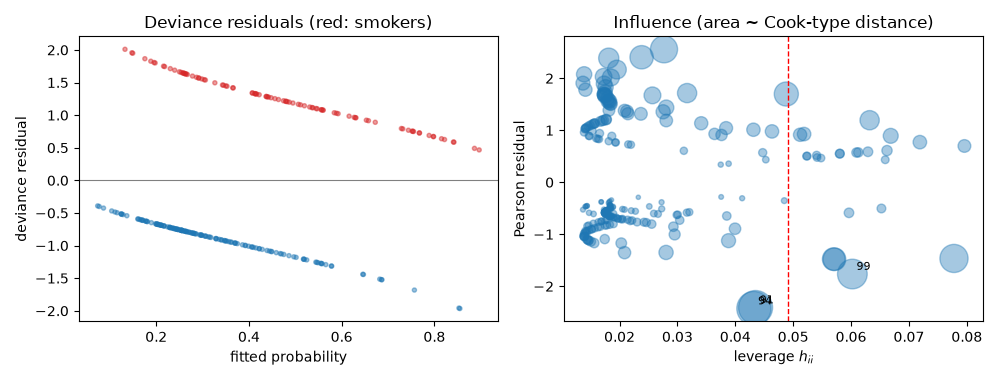
\includegraphics[width=0.98\linewidth]{fig_diag.png}

    \vspace{0.2em}
    {\scriptsize
    \begin{tabular}{@{}rlrrrrr@{}}
      \toprule
      row & day, size, $y$ & $\hat\pi$ & $r_P$ & $h_{ii}$ & $\Delta$dev & Cook \\
      \midrule
      $94$  & Fri, 2, 0 & $0.855$ & $-2.43$ & $0.043$ & $4.14$ & $0.055$ \\
      $91$  & Fri, 2, 0 & $0.853$ & $-2.41$ & $0.044$ & $4.11$ & $0.055$ \\
      $187$ & Sun, 5, 1 & $0.133$ & $+2.56$ & $0.028$ & $4.23$ & $0.035$ \\
      \bottomrule
    \end{tabular}}
  \end{column}
  \begin{column}{0.44\textwidth}
    \small
    \begin{itemize}
      \item $r_P=(y-\hat\pi)/\sqrt{\hat\pi(1-\hat\pi)}$; deviance residuals
            $\pm\sqrt{-2\ln\hat\pi\ \text{or}\ -2\ln(1-\hat\pi)}$; largest
            $|r_P|=2.56$.
      \item Leverage from the weighted hat matrix: $24$ of $244$ cases above $2p/n=0.049$.
      \item Influence by exact case deletion ($\Delta$deviance, Cook-type
            distance): largest $0.055$; the one-step formula agrees
            (correlation $0.997$).
      \item The worst cases are \emph{Friday non-smokers} in a mostly-smoking
            baseline: no case drives the fit.
    \end{itemize}
  \end{column}
  \end{columns}
\end{frame}

% ===================== 6. CLASSIFICATION ============================
\begin{frame}{6. Classification: cutoffs, ROC and AUC}
  \begin{columns}[T]
  \begin{column}{0.52\textwidth}
    \centering
    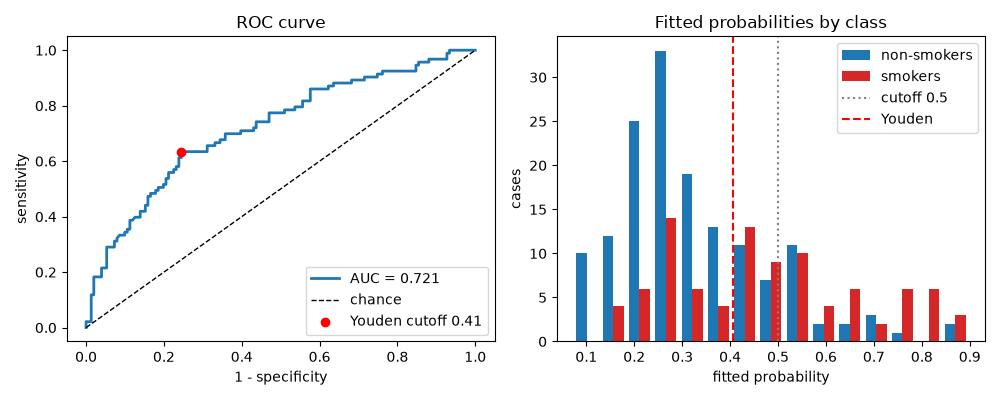
\includegraphics[width=0.98\linewidth]{fig_roc.png}

    \vspace{0.2em}
    \raggedright\small
    AUC $=0.721$ in sample; on $190$ random $50/50$ splits $0.690$
    (bill only $0.518$, bill+size $0.608$, day only $0.657$). Ten splits were
    dropped: the training half separated.\par
  \end{column}
  \begin{column}{0.48\textwidth}
    \small
    {\scriptsize\setlength{\tabcolsep}{3pt}
    \begin{tabular}{@{}lrrrr@{}}
      \toprule
      cutoff & sensit. & specif. & precis. & accur. \\
      \midrule
      $0.50$            & $0.419$ & $0.854$ & $0.639$ & $0.689$ \\
      $0.381$ (base rate) & $0.634$ & $0.715$ & $0.578$ & $0.684$ \\
      $0.407$ (Youden)  & $0.634$ & $0.755$ & $0.615$ & $0.709$ \\
      \bottomrule
    \end{tabular}}

    \vspace{0.4em}
    \begin{itemize}
      \item At $0.5$ the model catches only $42\%$ of smokers; the Youden cutoff $0.407$
            gives $63\%$ at accuracy $0.709$.
      \item The rule ``nobody smokes'' is already $0.619$ accurate: accuracy
            flatters this model.
      \item AUC is the probability that a random smoker gets a higher $\hat\pi$
            than a random non-smoker.
    \end{itemize}
  \end{column}
  \end{columns}
\end{frame}

% ===================== 7. LINKS, SEPARATION, POISSON, GLM ===========
\begin{frame}{7. Separation, other links, Poisson regression, GLMs}
  \begin{columns}[T]
  \begin{column}{0.52\textwidth}
    \small
    \key{Separation:} no party of $6$ smokes ($0/4$); an indicator for
    \texttt{size}$=6$ has no finite ML coefficient: $-1.9,\,-5.1,\,-11.2,\,-21.2,\,-41.2$
    after $1,\,4,\,10,\,20,\,40$ iterations, $se\approx4\times10^{8}$.
    A data problem, not a model error (Firth, merge classes).

    \vspace{0.3em}
    \key{Links} (same linear predictor): $AIC$ $298.74$ (logit), $298.81$
    (probit), $299.23$ (cloglog); logit/probit coefficient ratio $\approx1.67$;
    max difference in $\hat\pi$ logit--probit $0.009$.

    \vspace{0.3em}
    {\scriptsize\setlength{\tabcolsep}{3pt}
    \begin{tabular}{@{}llll@{}}
      \toprule
      model & response & distribution & link \\
      \midrule
      linear   & continuous & normal   & identity \\
      logistic & binary     & binomial & logit \\
      Poisson  & count      & Poisson  & log \\
      \bottomrule
    \end{tabular}}
  \end{column}
  \begin{column}{0.48\textwidth}
    \centering
    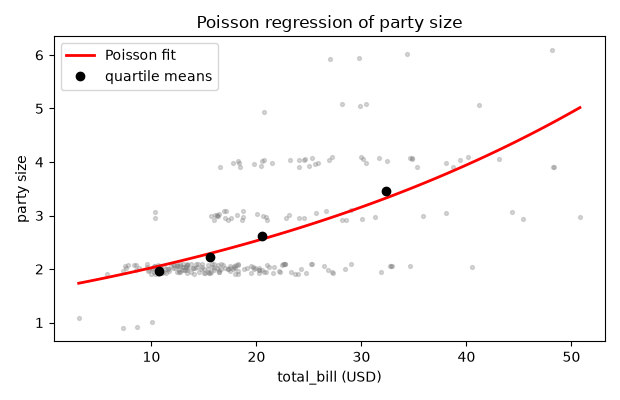
\includegraphics[width=0.84\linewidth]{fig_poisson.png}

    \vspace{0.1em}
    \raggedright\scriptsize
    \key{Poisson:} party size on bill, $\ln\mu=0.483+0.0222\,$bill; rate ratio
    $1.249$ per $10$~USD ($1.154$--$1.352$). Pearson $\chi^2/df=0.21$: size is
    \emph{under}dispersed (and never $0$), so the Poisson se ($0.0040$) is
    conservative (quasi-Poisson $0.0019$).\par
  \end{column}
  \end{columns}
\end{frame}

\end{document}
